
\section{The Proposed \method}

In this section, we describe the details of \method approach for solving long-context tasks, including the overall workflow ($\mathsection$~\ref{sec:workflow}), Multi-conv RL algorithm for training \method ($\mathsection$~\ref{sec:training}), reward modeling design ($\mathsection$~\ref{sec:reward}), and architecture implementation design ($\mathsection$~\ref{sec:architecture}).

\subsection{The \method Workflow: RL-shaped Memory for Unbounded Contexts}
\label{sec:workflow}

% \paragraph{\textbf{From unbounded streams to bounded thinking.}}
As illustrated in \autoref{fig:workflow}, \method views an arbitrarily long document not as a monolithic block but as a controlled {\it stream} of evidence.
At every step, the model sees exactly two things: the next chunk of text and a compact, fixed-length \textit{memory} that summarizes everything deemed important so far.
Crucially, the memory is just a sequence of ordinary tokens inside the context window, so the core generation process of the base LLM remains unchanged.

% \paragraph{\textbf{Overwrite\,\&\,refine—an RL-tuned strategy.}}
After reading a new chunk, the model overwrites the previous memory with an updated one.
This \textbf{overwrite} strategy seems almost too simple, yet it is precisely what enables the system to scale:
because memory length never grows, the total compute per chunk stays $O(1)$ and end-to-end complexity is strictly linear to the number of chunks.
We formulate the overwrite decision as a reinforcement learning problem: the agent is rewarded for retaining information that will later prove useful and for discarding distractors that would waste precious tokens.
By optimizing this objective with our newly introduced multi-conversation DAPO algorithm (detailed in $\mathsection$~\ref{sec:training}), the model learns to compress aggressively while preserving answer-critical facts.

The workflow naturally decomposes inference into two modules.
Within the \textbf{Context-Processing} module the model iterates over chunks, updating memory with a prompt template (Table~\ref{tab:template}, top).
Once the stream is exhausted, a final \textbf{Answer-Generation} module is invoked (Table~\ref{tab:template}, bottom) where the model consults only the problem statement and the memory to produce its boxed answer.
Because positional embeddings are never re-scaled or patched, the same tokenization and attention layout apply in both modules, unlocking the model's latent length-extrapolation capability without any architectural modifications.

\method therefore enjoys three benefits from this design:
(1) {\textbf{Unlimited length}: the document can be millions of tokens because it is processed as a stream;
(2) {\textbf{No performance cliff}: RL encourages the memory to retain exactly the information needed, yielding near-lossless extrapolation (Figure~\ref{fig:front});
(3) {\textbf{Linear cost}: a constant window size implies decoding time and memory consumption grow linearly with input length ($O(N)$) (detailed in $\mathsection$~\ref{sec:training}.)
This renders a practical recipe for turning any moderately context-sized LLM into an efficient long-context reasoner with minimal engineering overhead.

\begin{table}[t]
  \centering
  \renewcommand{\arraystretch}{1.1}
  \begin{tabularx}{\textwidth}{>{\raggedright\arraybackslash}X}
    \toprule
    % ------------------------ Context-processing prompt ------------------------
    You are presented with a \textbf{problem}, a \textbf{section} of an article that
    may contain the answer, and a \textbf{previous memory}.  
    Please read the section carefully and \emph{update the memory} with new
    information that helps to answer the problem, while retaining all relevant
    details from the previous memory.\\[4pt]

    \texttt{<problem>} 
    \texttt{\{prompt\}} 
    \texttt{</problem>} \\[2pt]

    \texttt{<memory>} 
    \texttt{\{memory\}} 
    \texttt{</memory>} \\[2pt]

    \texttt{<section>} 
    \texttt{\{chunk\}} 
    \texttt{</section>} \\[4pt]

    \textbf{Updated memory:}\\
    \midrule
    % ------------------------ Answer-generation prompt ------------------------
    You are presented with a \textbf{problem} and a \textbf{previous memory}.
    Please answer the problem based on the previous memory and put the answer in
    \verb|\boxed{}|.\\[4pt]

    \texttt{<problem>} 
    \texttt{\{prompt\}} 
    \texttt{</problem>} \\[2pt]

    \texttt{<memory>} 
    \texttt{\{memory\}} 
    \texttt{</memory>} \\[4pt]

    \textbf{Your answer:}\\
    \bottomrule
  \end{tabularx}
  \caption{Template of \method{} for context processing (top part) and final
  answer generation (bottom). Curly-brace placeholders \{\} will be replaced
  with actual content.}
  \label{tab:template}
\end{table}

\subsection{Training \method with Multi-conv RL}
\label{sec:training}

By viewing memory update in context processing for answer-generation tasks as part of the policy to be optimized by RL, we adopt the RLVR recipe~\cite{o1,guo2025deepseek,seed2025seed1} to train \method.


For the base algorithm, we adopt Group Relative Policy Optimization (GRPO)~\cite{deepseekmath} for its simplicity and effectiveness in RLVR. 
In the rollout phase of GRPO, the policy model $\pi_{\theta_\text{old}}$ samples a group of $G$ individual responses $\{ o_i\}_{i=1}^G$ for an input $x$. Let $\{ R_i \}_{i=1}^G$ refer to the sequence-level rewards, then the group normalizing advantage of the $i$-th response is calculated by the following function:
\begin{equation}
\hat{A}_{i,t} = \frac{r_i - \text{mean}(\{R_i\}_{i=1}^G)}{\text{std}(\{R_i\}_{i=1}^G)}.
\end{equation}
GRPO adopts a clipped objective with a KL penalty term:

\begin{equation}
\begin{aligned}
\mathcal{J}_\text{GRPO}(\theta)& = \mathbb{E}_{(q,a)\sim \mathcal{D}, \{o_i\}_{i=1}^G\sim \pi_{\theta_\text{old}}(\cdot\mid q)} \\&
\Bigg[ \frac{1}{G}\sum_{i=1}^{G} \frac{1}{|o_i|}\sum_{t=1}^{|o_i|} \Bigg( 
\min \Big( r_{i,t}(\theta) \hat{A}_{i,t},  
\ \text{clip} \Big( r_{i,t}(\theta), 1 - \varepsilon, 1 + \varepsilon \Big) \hat{A}_{i,t} \Big)
- \beta D_{\text{KL}}(\pi_{\theta} || \pi_{\text{ref}}) 
\Bigg) \Bigg],
\label{eq:grpoloss}
\end{aligned}
\end{equation}
where $r_{i,t}(\theta)$ refers to the importance sampling weight: 
\begin{equation}
    r_{i,t}(\theta)=\frac{\pi_{\theta}(o_{i,t} \mid q, o_{i,<t})}{\pi_{\theta_{\text{old}}}(o_{i,t} \mid q,o_{i,<t})}.
\end{equation}

However, due to the nature of the \method approach, it generates multiple context-independent conversations for a single query, as illustrated in \autoref{fig:workflow}. Therefore, policy optimization cannot be implemented by simply applying the attention mask as is done in multi-turn tool-calling optimization.


To address this issue, we treat each conversation as an independent optimization target, as demonstrated in \autoref{fig:rl}. Let $n_i$ denote the number of generated conversations $ (o_{i,1}, o_{i,2}, ..., o_{i,n_i})$ for a given sample $(q_i, a_i)$ in a group. $o_{i,j}$ further decomposes into token-level outputs $(o_{i,j,1}, o_{i,j,2}, ..., o_{i,j,|o_{i,j}|})$. We compute an outcome reward $R_i$ per sample by the final conversation that contains the final answer,  and distribute group-normalized advantages across all associated conversations.

\begin{figure}
    \centering
    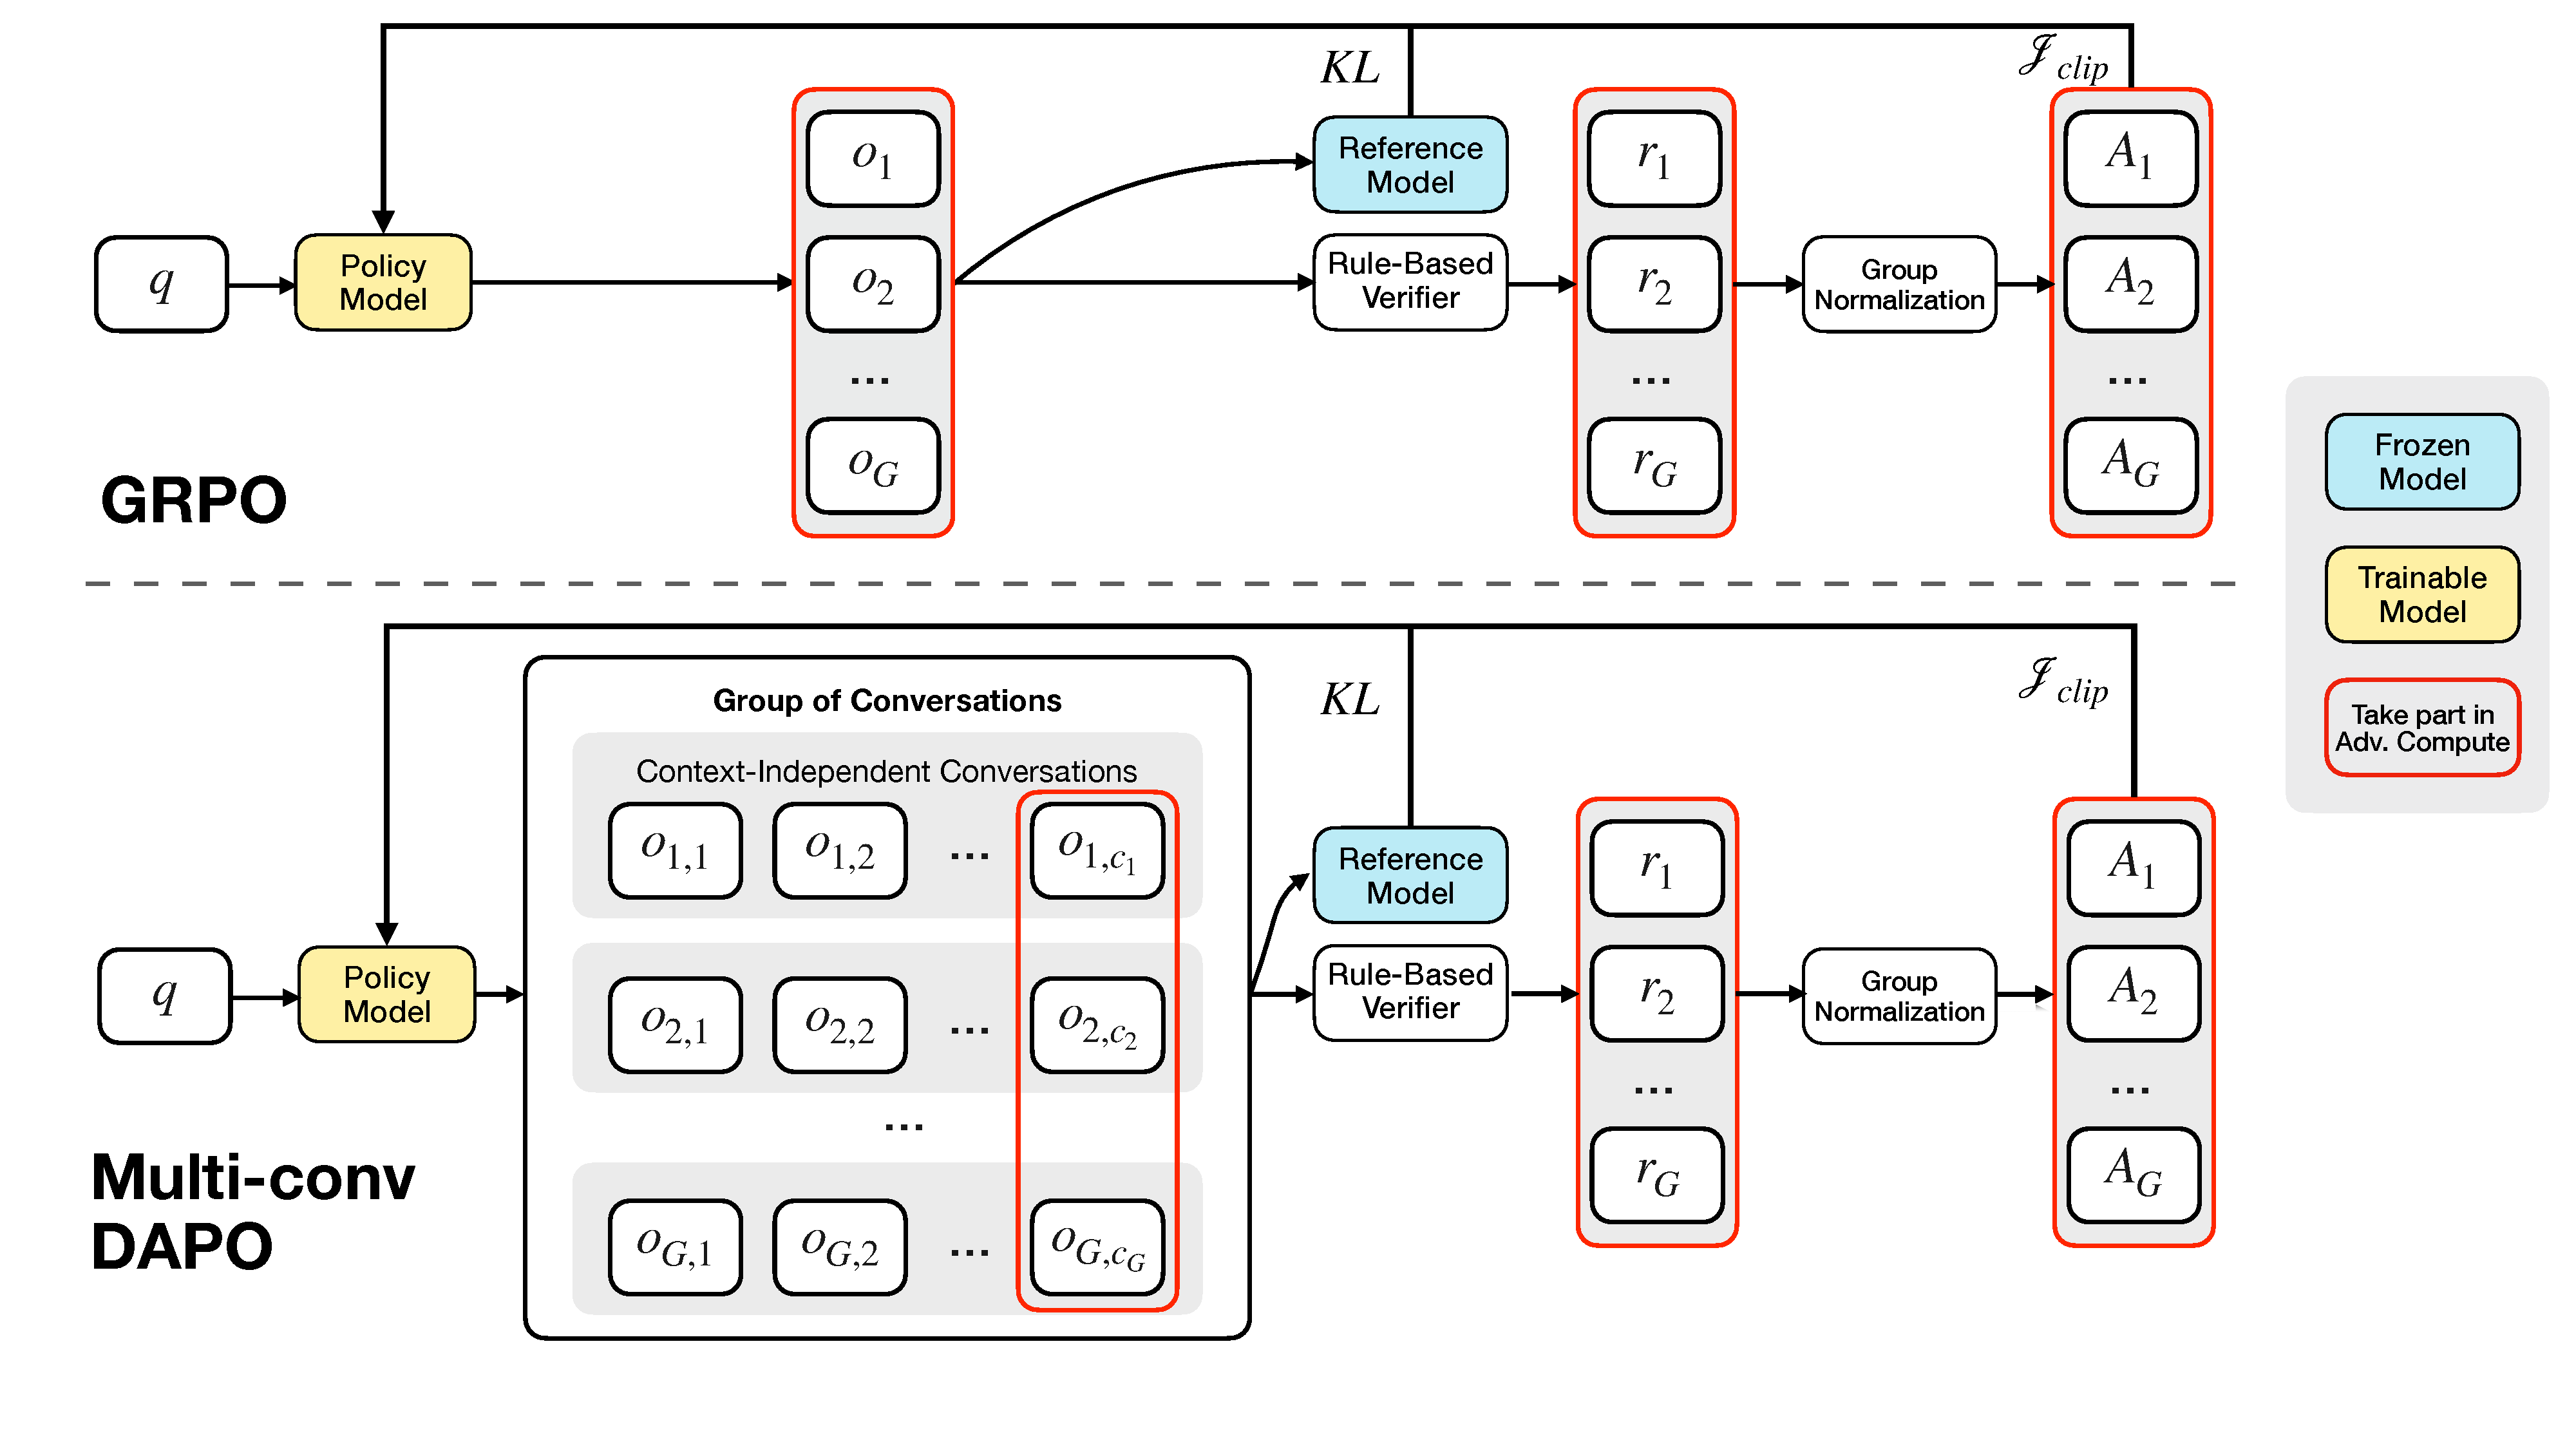
\includegraphics[width=0.9\linewidth]{figs/algo.pdf}
    \caption{Comparison between vanilla GRPO and Multi-Conv DAPO. During the rollout phase of Multi-conv DAPO, each sample generates multiple conversations. The answer contained in the final conversation is used to compute the reward and advantage, which are then employed to optimize all preceding conversations.}
    \label{fig:rl}
\end{figure}


Equations~\ref{eq:adv_multiconv} and \ref{eq:loss_multiconv} illustrate how the advantage and loss are computed within our \method algorithm for context-independent multi-conversation rollouts. 
The advantage value is derived from the conversation that contains the final answer, then uniformly applied across all conversations originating from the same sample. Our loss function is analogous to that used in DAPO~\cite{yu2025dapo}, which incorporates a token-level averaging loss. Furthermore, we extend the dimensionality of the loss computation from the conventional \texttt{(group, token)} structure to \texttt{(group, conversation, token)}. Following DrGRPO~\cite{liu2025understanding}, we do not normalize the advantage by the standard deviation of rewards.

\begin{equation}
\hat{A}_{i,j,t} = r_i - \text{mean}(\{R_i\}_{i=1}^G)
\label{eq:adv_multiconv}
\end{equation}

\begin{equation}
\begin{aligned}
\mathcal{J}_{\text{DAPO}}(\theta) = \quad&\mathbb{E}_{(q,a)\sim \mathcal{D}, \{o_{i,j}\}_{i=1}^G\sim \pi_{\theta_\text{old}}(\cdot\mid q,~o_{i,j-1})}\\&
\Bigg[\frac{1}{\sum_{i=1}^{G}\sum_{j=1}^{n_i}|o_{i,j}|}\sum_{i=1}^{G}\sum_{j=1}^{n_i}\sum_{t=1}^{|o_{i,j}|}
 \Big(\mathcal{C}_{i,j,t} - \beta D_{\text{KL}}(\pi_{\theta} || \pi_{\text{ref}} \Big) \Bigg]
\\
\text{where\quad} \mathcal{C}_{i,j,t} = &\min\Big(r_{i,j,t}(\theta) \hat{A}_{i,j,t},  
\ \text{clip} \Big( r_{i,j,t}(\theta), 1 - \varepsilon_{low}, 1 + \varepsilon_{high} \Big) \hat{A}_{i,j,t}\Big)
\label{eq:loss_multiconv}
\end{aligned}
\end{equation}

\subsection{Reward Modeling}
\label{sec:reward}
Following the RLVR recipe~\cite{guo2025deepseek, jin2025search, yu2025dapo},
we train the model with a final outcome reward computed by a rule-based verifier. 
In RULER~\cite{hsieh2024ruler} and other datasets, questions may have multiple ground-truth answers. 
For some tasks, such as question answering, these ground truths are considered equivalent. Given a set of multiple ground-truth answers $Y = \{y_1, y_2, \dots, y_n\}$, the reward score is defined as:
\begin{equation}
R(\hat{y}, Y) = \max_{y \in Y} \big(\mathbb{I}( \texttt{is\_equiv}(y,\hat{y})\big)
\end{equation}
where $\hat{y}$ is the predicted answer, and $\mathbb{I}(\cdot)$ denotes the indicator function.

For other tasks, all ground-truth answers are expected to be included in the final output. An example is the task of Multi-Value Needle in a Haystack, where the question might be: ``What are all the special magic numbers for XXX?'' 
In such cases, the reward function is defined as:
\begin{equation}
R(\hat{y}, Y) = \frac{|{y \in Y \mid \mathbb{I}(y \in \hat{y})}|}{|Y|}
\end{equation}
where $|\cdot|$ denotes the cardinality of a set.

\subsection{Rethinking \method from Autoregressive Modeling Perspectives}
\label{sec:architecture}

Finally, to get a deeper sense of the \method design, we propose to re-think language-model factorization in the following fashion.  
A standard autoregressive LLM factorizes the joint likelihood of a sequence $\mathbf{x}_{1:N}$ as
\(
p(\mathbf{x}_{1:N})=\prod_{n=1}^N p(x_n\mid\mathbf{x}_{1:n-1}),
\)
implicitly assuming that every past token (or at least its hidden state) must stay in the active context.
This is what turns quadratic attention into the long-context bottleneck.

\method replaces the unbounded history with a fixed-length {\it memory} $\mathbf{m}\!\in\!\mathbb{V}^M$, as shown in Figure~\ref{fig:arch}.
The input text is streamed through the model in $K$ contiguous chunks
$\mathbf{c}^1,\dots,\mathbf{c}^K$ (each of length $\le C$).
After chunk $k$ is read, the model overwrites the panel with a new vector $\mathbf{m}^k$ that summarizes {\it all} evidence seen so far.
Because $|\mathbf{m}^k|=M$ is constant, both compute and memory per step are $O(C+M)$, yielding an overall linear complexity $O(N)$.


Introducing the latent sequence $\mathbf{m}^{1:K-1}$ decomposes the original likelihood as
\begin{align}
p(\mathbf{x}_{1:N})
&=\!\!\!\!\sum_{\mathbf{m}^{1:K-1}}
\prod_{k=1}^{K}
\underbrace{p(\mathbf{c}^k\mid\mathbf{m}^{k-1})}_{\text{read}}
\;\underbrace{p(\mathbf{m}^k\mid\mathbf{c}^k,\mathbf{m}^{k-1})}_{\text{write}}, \label{eq:marl}
\end{align}
with base case $\mathbf{m}^0=\varnothing$.
Inside each chunk, we still run an ordinary transformer decoder, but conditioned on a {\it constant} context window
$(\mathbf{c}^k,\mathbf{m}^{k-1})$.
The read path factorizes token-by-token,
\(
p(\mathbf{c}^k\mid\mathbf{m}^{k-1})
    =\!\!\!\prod_{i=(k-1)C+1}^{kC} \!p(x_i\mid\mathbf{x}_{1:i-1},\mathbf{m}^{k-1}),
\)
while the write path generates the next memory in the same autoregressive fashion.

\begin{figure}[t]
    \centering
    
\includegraphics[width=0.9\linewidth]{figs/arch.pdf}
    \caption{The architecture and graphic model of \method. The memory is modeled as a latent memory variable, thereby enabling the decomposition of the autoregressive language model into multiple steps of reading from and writing to the memory.
 }
    \label{fig:arch}
\end{figure}

\method enjoys token-level compression of context, yet local-global or linear-attention models compress long context in the {\it feature} space; their summaries are implicit and opaque.
\method's summaries reside in token space, so every intermediate memory is human-readable and can be inspected or even edited — a property we exploit when designing the RL reward (§\ref{sec:reward}).
Conceptually, Equation~\ref{eq:marl} turns the transformer into a recurrent network whose state size is user-controllable.

\textbf{Why is RL Essential?}
Because memory tokens are latent and updated via a discrete overwrite rule, back-propagation alone cannot teach the model {\it what} to keep and what to discard.
Our multi-conversation GRPO algorithm (§\ref{sec:training}) treats each read–write–read loop as an RL transition, directly rewarding memories that lead to a correct final answer.
This bridges the gap between explicit supervision (answers) and implicit structure (good memories), completing the training pipeline introduced earlier.


The resulting \method architecture preserves the vanilla decoder's training recipe, requires no exotic attention kernels, and satisfies the long-context trilemma of arbitrary length, lossless extrapolation, and linear cost.
